\documentclass{scrartcl}

\usepackage[ngerman]{babel}

\usepackage[utf8]{inputenc}
\usepackage{hyperref,xcolor,microtype,ifthen}
\usepackage{csquotes}

\usepackage{graphicx}
\usepackage{svg}

\usepackage{helvet}
\renewcommand{\familydefault}{\sfdefault}
\fontfamily{phv}\selectfont

\linespread{1.25}

\title{Mobile Application Lab}
\subtitle{Dokumentation}
\date{07.03.2018}
\author{Max Landthaler,Manuel Konstantin Hinke}

\begin{document}

\maketitle

\section{Einleitung}
\subsection{Motivation}


Im Rahmen des Anwendungsfaches Mobile Application Lab wurde eine Quartett App geschrieben. Ziel des ganzen war es einen grundlegenden Einstieg in die Android Programmierung zu finden. Da ein Spiel viele verschiedene Bereiche abdeckt eignet es sich ideal für den Lernprozess.
Übergeordnete Motivation war der Lernprozess wofür sich dieses Szenario sehr gut eignet.

\subsection{Ziel}

Das hiermit erklärte Ziel dieses Projekts ist die Entwicklung einer Quarett-App fortwährend auch Unicorn-Quartett genannt. Es sollen gängige und Vorgehensweisen und Best Practices erarbeitet werden.
Dabei ist auch Ziel herauszufinden welche Schwierigkeit es gibt beim Implementieren für Android Betriebsysteme unterschiedlicher Versionen zu entwickeln.


\subsection{Aufbau}

Die folgende Dokumentation beschreibt den Enwicklungs und Implementierungsablauf.
Dabei werden zuerst Grundlegende Rahmen definiert und eine Anforderungsanalyse erstellt, die sowohl funktionale als auch nicht funktionale Anforderungen erfüllt.
Auch das erdachte Design und Struktur Konzept wird beschrieben um auch eventuell vergleichen zu können wo sich das Endresultat mit dem tatsächlich erreichten unterscheidet.
Es folgen dann ausgewählte Implementierungsdetails und abschließend ein Abgleich der Anforderungen.

\section{Grundlagen}
\subsection{Quartettspiel}

Beim klassischen Quartett geht das darum, möglichst viele Quartette (Ansammlung von 4 Karten gleicher Kategorie) zu erspielen.
Dabei werden die Werte der Kontrahenten verglichen und der höhere Wert gewinnt. Der Gewinner bekommt die unterlegenden Karten.
Das Unicorn-Quartet spielt im Standardmodus eine Abwandlung des klassischen Quartetts, das sich Supertrumpf nennt bzw. im Umgangssprachlichen als
Autoquartett  bezeichnet wird. Es folgen die genauen Beschreibungen der Spielelemente und Spielmodi.
\subsubsection{Quartettkarte}

\begin{figure}[!ht]
\begin{center} 
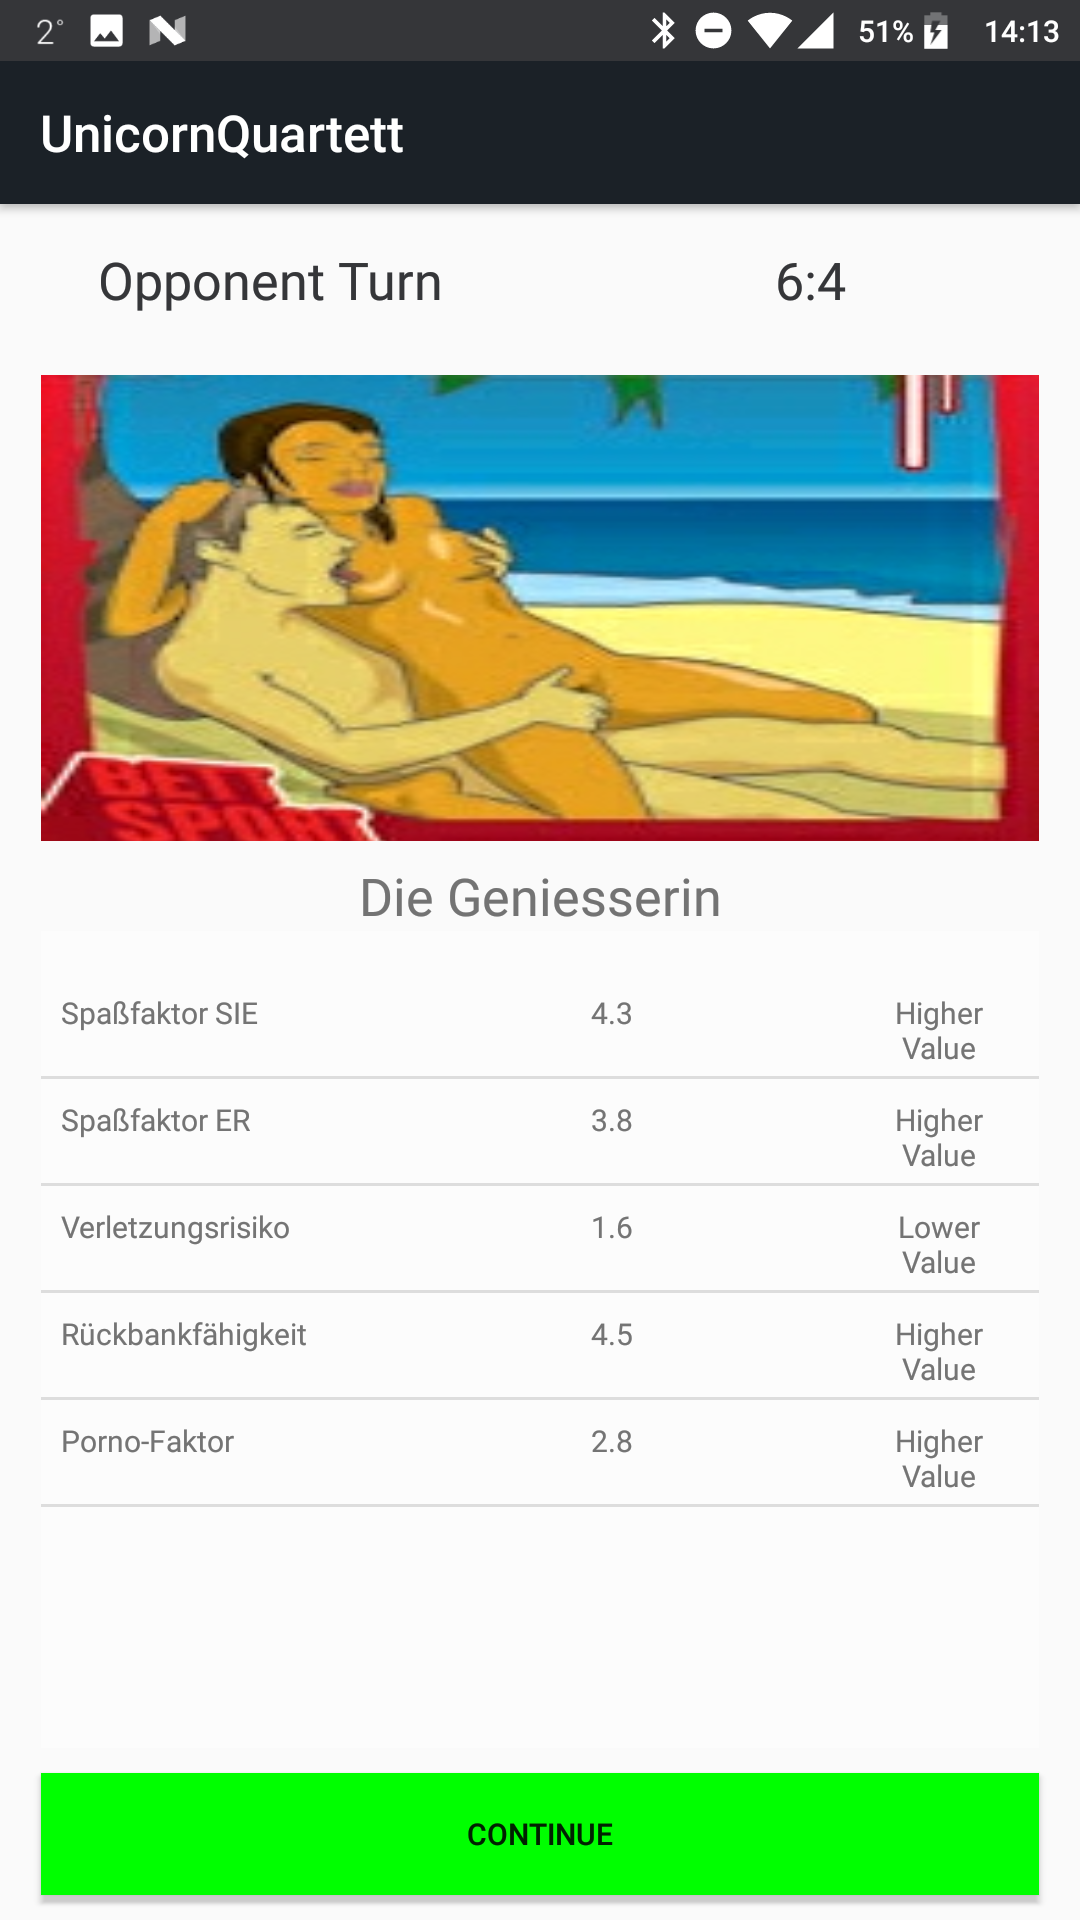
\includegraphics[scale=0.1]{pics/QuartettKarte.png}
    \caption{Die Geniesserin  aus dem Bettsport Deck}
\end{center}
\end{figure}

In Abb.1 wird eine Quartettkarte im Unicorn-Quartett visualisiert.
Ganz oben wird der aktuelle Spielstand angezeigt und wer aktuell am Zug ist.
Dann folgt ein Bild, auf dem das entsprechende Objekt der Karte zu sehen ist, in diesem Fall ein Auto.
Unten werden die zur Auswahl stehenden Werte angezeigt.


\subsubsection{Spielverlauf}
An einem Spiel nehmen der Spieler und eine Künstliche Intelligenz als Kontrahent teil.
Der menschliche Spieler legt ein Quartett und den Spielmodus fest.
Hierbei kann sich zwischen einem normalen Spiel und dem sog. Unicorn Modus entscheiden.
Zu Spielbeginn werden die Karten des Quartetts gemischt und gleichmäßig an die beiden Kontrahenten verteilt.
Der menschliche Spieler ist immer zuerst an der Reihe und wählt einen Wert von seiner aktuellen Karte aus, mit dem er seinen Kontrahenten stechen möchte.
Nachdem er seinen Wert bestätigt hat, werden sein Wert und der des Kontrahenten verglichen. Wer den besseren Wert hatte, bekommt die Karte des Verlierers.
Anschließend ist der andere Spieler an der Reihe, d.h. es wird unabhängig vom Ausgang der vorheringen Runde immer abgewechselt.
Gewinner des Spiels ist ganz klassisch der Spieler, der am Ende alle Karten hat.
\newline
Um etwas Abwechslung in den normalen Quartett Spielfluss zu schaffen, wurde der Unicorn Modus entwickelt.

\subsubsection{Spielmodi}

\textbf{Normal:}
Der klassische Modus. Hier wird abwechselnd gespielt. Gewonnen hat derjenige, der am Ende alle Karten hat.
\newline
\textbf{Unicorn}:
Der überraschende Modus. Auch hier wird abwechselnd gespielt. Jedoch können beide Kontrahenten ab einer Siegesserie von 3 hintereinander gewonnen Runden, sofern sie selbst
an der Reihe sind, besondere, zufällig generierte Aktionen ausführen, die zu ihrem direkten Vorteil sind.
Außerdem werden zufällig generierte Events, die beide Spieler positiv oder negativ beeinflussen, in das Spiel gestreut, ohne dass die Spieler darauf Einfluss nehmen können.
Gewonnen hat der Spieler, der alle Karten hat oder die richtige Aktion ausgespielt hat.


\subsection{Mobile Anwendungen}
Ziel dieses Projektes war es, sich mit der Entwicklung von mobilen Anwendungen auf einer beliebigen Plattform zu befassen und erste Erfahrungen zu sammeln.

Da beide Entwickler ein Android Endgerät besitzen und auch Interesse an dieser Umgebung haben, war sofort Android als Plattform gesetzt.
 
Weitere Vorteile bei der Entwicklung von Android Anwendungen sind die große Verbreitung von Android Endgeräten und die Verwandtheit zur normalen Java Entwicklung.

Im Hinblick auf mobile Anwendungen fallen besonders die beschränkten Ressourcen wie begrenzte Akkukapazität, Arbeitsspeicher, Rechenleistung und Festplattenspeicher ins Gewicht.
Im Vergleich zu normalen PCs oder Servern stehen auf einem mobilen Gerät viel weniger Ressourcen zur Verfügung, die zudem von vielen Anwendungen sowie dem System gleichzeitig verwendet werden.

\subsection{Libraries und Frameworks}
Um einige Funktionen der Applikation nicht selbst implementieren zu müssen
wurden folgende zusätzliche Programmbibliotheken und Frameworks verwendet:

\noindent
\newline 
\textbf{Volley, https://github.com/google/volley} \newline
Volley ist eine Bibliothek, die es sich zur Aufgabe gemacht hat, Netzwerkoperationen sehr einfach und effektiv durchzführen.
Mithilfe von Volley wurde das Downloaden von neuen Decks und Karten realisiert.

\ \newline
\textbf{CircleImageView, https://github.com/hdodenhof/CircleImageView} \newline
Hiermit wird eine runde ImageView eingeführt, die für die Abbildung des Profil Bildes verwendet wurde.

\ \newline
\textbf{Realm, https://github.com/realm/realm-java} \newline
Realm ist eine objektorientiere Datenbank, die sich gerade für Android eignet, um einfach und ohne echte Datenbankbefehle tatsächliche Objekte in einer Datenbank zu verwalten, was die Behandlung der einzelnen Spielstatistiken und Decks sowie deren Karten, Attribute und Bilder sehr einfach gestaltet. 


\section{Anforderungsanalyse}
\subsection{Funktionale Anforderungen}

Ein wichtiges Thema im Vorfeld der Implementierung war es die Anforderungen an das Unicorn Quartett klar zu definieren.
Im folgenden werden die funktionalen und nicht funktionalen Anforderungen
aufgelistet, die vor der Entwicklung der Applikation formuliert wurden. 
\ \pagebreak

\textbf{FA1 Ladebildschirm} \newline
Beim Öffnen der App erscheint ein Ladebildschirm, in dem das Logo der App dargestellt wird. Zudem befindet sieht der Nutzer eine Fortschrittsanzeige mit Statusmeldungen. Anschließend wird der Nutzer automatisch auf den Startbildschirm weitergeleitet.
\ \newline
\textbf{FA1-0 Nutzer erstellen} \newline
Wenn der Nutzer zum ersten Mal die App startet, wird er dazu aufgefordert, einen Benutzer zu erstellen. Dies muss zu beim Start der App getätigt werden. Zur Erstellung des Nutzer wird ein Name und ein Profilbild welches wahlweise mit der Kamera aufgenommern werden kann oder aus der Galerie ausgewählt werden kann, benötigt. Über den Namen kann der Nutzer von anderen Nutzern identifiziert werden.
\ \newline
\textbf{FA1-1 Startbildschirm} \newline
Auf dem Startbildschirm befinden sich 5 Elemente: Über Buttons mit entsprechenden Icons gelangt der Nutzer zu den folgenden Ansichten:
- Spielen
- Kartenverwaltung/Kartengallerie
- Freunde
- Rangliste
- Profil
\ \newline
\textbf{FA2-1 Spiel erstellen | Offline Spiel} \newline
Auf der Spielansicht kann der Nutzer zwischen  zwei Optionen wählen:
- Offline Spiel gegen die „KI“
- Online Spiel gegen Freunde
Nach der Auswahl gelangt der Spieler auf die Ansicht, in der er sich zwischen den verschiedenen entscheiden kann.
\ \newline
\textbf{FA2-2 Online Spiel} \newline
Wählt der Spieler die Option „online“ aus, kann er entweder gegen einen zufällig ausgewählten Online-Spieler spielen oder er wählt einen Spieler aus seiner Freundesliste aus.
\ \newline
\textbf{FA2-3 Spielmodi} \newline
Der Nutzer kann zwischen zwischen zwei Spielmodi auswählen:
\ \newline
- Standard (Stechen) 
\ \newline
- Unicorn Mode (Stechen, aber mit globalen Events und Sonderkarten)
\ \newline
\textbf{FA2-4 Spiel} \newline
Im eigentlichen Spiel sieht der Spieler je Runde genau eine Karte mit aktuellem Bild und den Werten der Karte. Der Nutzer wählt einen Wert aus, der ihm am vielversprechendsten erscheint.
Dann erfolgt ein Wechsel der Anzeige von der einzelnen Karte des Spielers zu einer Gegenüberstellung der beiden Karten der gegeneinander antretenden Spieler. Der Wert des Siegers wird grün markiert, der des Verlierers rot. 
Der aktuelle Spielstand wird eingeblendet und die nächste Runde beginnt.
Dabei wird sichtbar visualisiert wer gerade am Zug ist.
\ \newline
\textbf{FA3-1 Kartenverwaltung} \newline
In der Kartenverwaltung wird dem Spieler eine Übersicht aller möglichen Decks angezeigt. Vorhandene Decks werden in Farbe abgebildet, Decks, die erst mit der Zeit erworben werden können, sind zu Beginn ausgegraut.
Klickt der Nutzer auf ein Deck, kann er sich die einzelnen Karten darin ansehen.
\ \newline\
\textbf{FA4-1 Bestenliste} \newline
In der Bestenliste werden die Top 5 Online Spieler angezeigt.
\ \newline
\textbf{FA5-1 Freunde} \newline
In der Freundesübersicht kann der Nutzer entweder einen Freund über seinen Namen hinzufügen oder kann die Liste seiner Freunde ansehen, wenn diese die Freundschaftsanfragen angenommen haben.
\ \newline
\textbf{FA6-1 Spieler Profil} \newline
Im Spielerprofil kann der Nutzer seinen Account mit Google verknüpfen, um seinen Fortschritt auch online zu speichern und um online spielen zu können.
Außerdem kann er hier seine Spielhistorie einsehen.
\ \newline

\subsection{Nicht Funktionale Anforderungen}
\ \newline
\textbf{NFA1 Aktuelle Version der Betriebssysteme} \newline
Die Oberfläche der App sollte sich an aktuelle Designrichtlinien orientieren und auf den gängigsten Versionen lauffähig sein.
\ \newline
\textbf{NFA2 Usability Ziele} \newline
Die App sollte einfach und verständlich aufgebaut werden sodass sich der Nutzer intuitiv in den Menüs zurechtfinden kann.
\ \newline
\textbf{NFA3 Feedback} \newline
Die App sollte dem Nutzer unter bestimmten Bedingungen ein Feedback geben.
Der Nutzer darf nie im Unklaren darüber sein was die App gerade macht.
\ \newline
\textbf{NFA4 Selbsterklärbarkeit} 
Die App sollte selbsterklärend aufgebaut sein. Der Nutzer sollte keine Probleme beim Verständnis der Funktionen oder Icons haben und ohne Hilfe das System bedienen können. Die App sollte ohne eine Anleitung bedienbar sein.
\ \newline
\textbf{NFA5 Benutzerfreundlichkeit} \newline
Die App sollte benutzerfreundlich aufgebaut sein, dass heißt der User soll einen positiven Eindruck von der App bekommen und sie gerne verwenden.
\ \newline
\textbf{NFA6 Verfügbarkeit} \newline
Die App sollte in den üblichen Smartphone Auflösungen darstellbar sein und sich auch an die Größenänderungen des Displays anpassen.
\ \newline
\textbf{NFA7 Robustheit} \newline
Die App sollte gegenüber Fehleingaben robust sein.
\ \newline
\textbf{NFA8 Reaktionszeit} \newline
Die App soll innerhalb so kurzer Zeit reagieren, dass der Nutzer keine nennenswerte Wartezeiten abwarten muss, ohne zu wissen, was vor sich geht.
\ \newline
\textbf{NFA9 Statusrückmeldung} \newline
Wenn die App nicht innerhalb angenehmer Reaktionszeiten reagieren kann, soll der Nutzer über eine aussagekräftige Anzeige über den aktuellen Zustand der App informiert werden.
\ \newline



\section{Konzept und Entwurf}
\subsection{Mockups}
Im Vorfeld der Implementierung musste natürlich auch ein Entwurfskonzept erarbeitet werden. Dieses Entwurfskonzept sollte die grundlegende Architektur der Applikation beschreiben und die einzelenen Screens in einer schlichten und funktionalen Art vorbereiten.
Wir haben bei der Erstellung dieser Screens auf eine softwareunterstütze Lösung verzichtet und haben diese per Hand erstellt.
\begin{figure}[!ht]
\begin{center}
	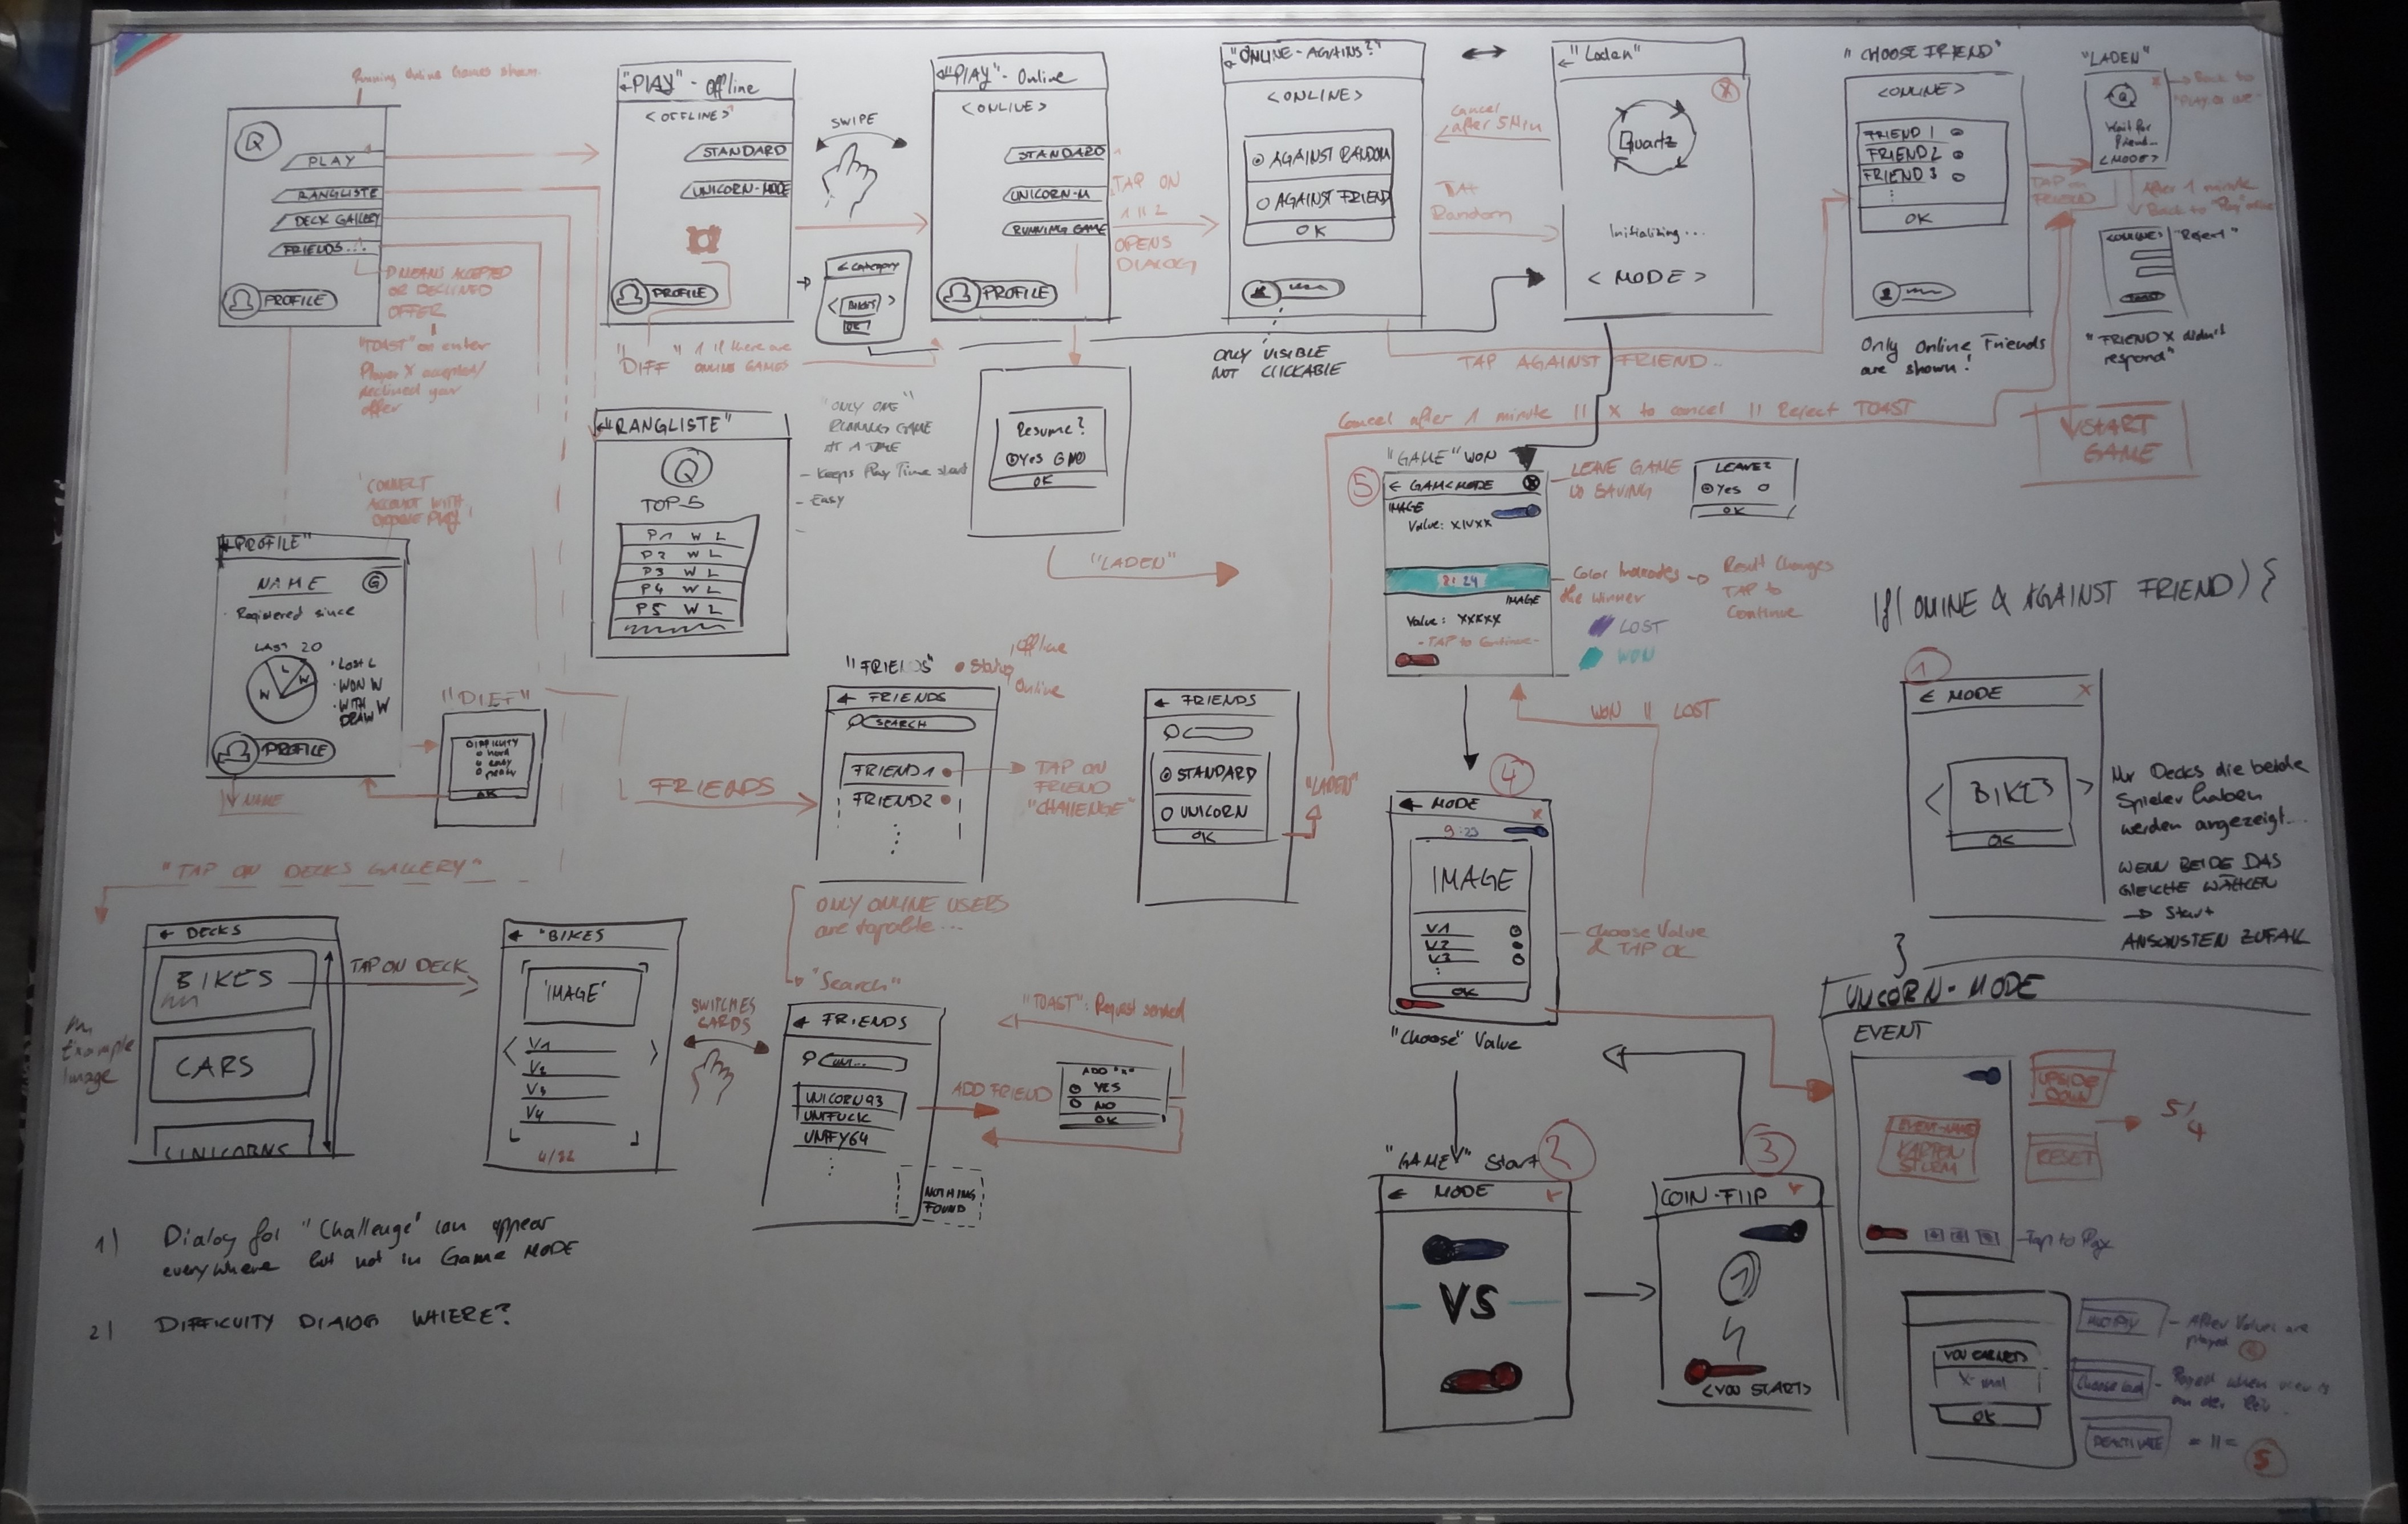
\includegraphics[scale=0.5]{pics/overview.png}
	\caption{Komplettansicht-Prozessablauf}
	\label{overview}
\end{center}
Darstellung der gesamten Möglichkeiten beziehungsweise Prozesse die in der App realisiert werden sollten. 
Das Profil ist von allen Screens aus erreichbar es sei denn man befindet sich in einem Spielprozess.
\end{figure}

\begin{figure}[!ht]
\begin{center}
	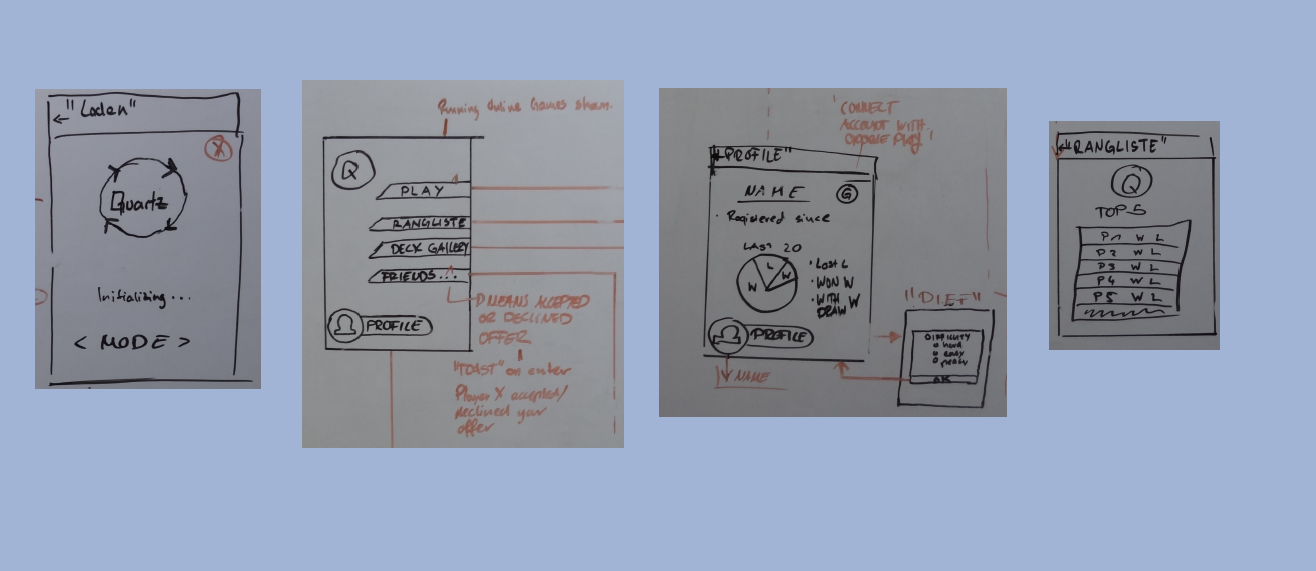
\includegraphics[scale=0.4]{pics/userhandling.png}
	\caption{Erstellung des Benutzers und bearbeiten der Daten}
	\label{UserProfil}
\end{center}
Abbildung ~\ref{UserProfil} skizziert den Prozess, welchen der Benutzer
vollführen muss, um einen Nutzer zu erstellen und wie er eingegebene Daten später wieder ändern kann.
\end{figure}

\begin{figure}[!ht]
\begin{center}
	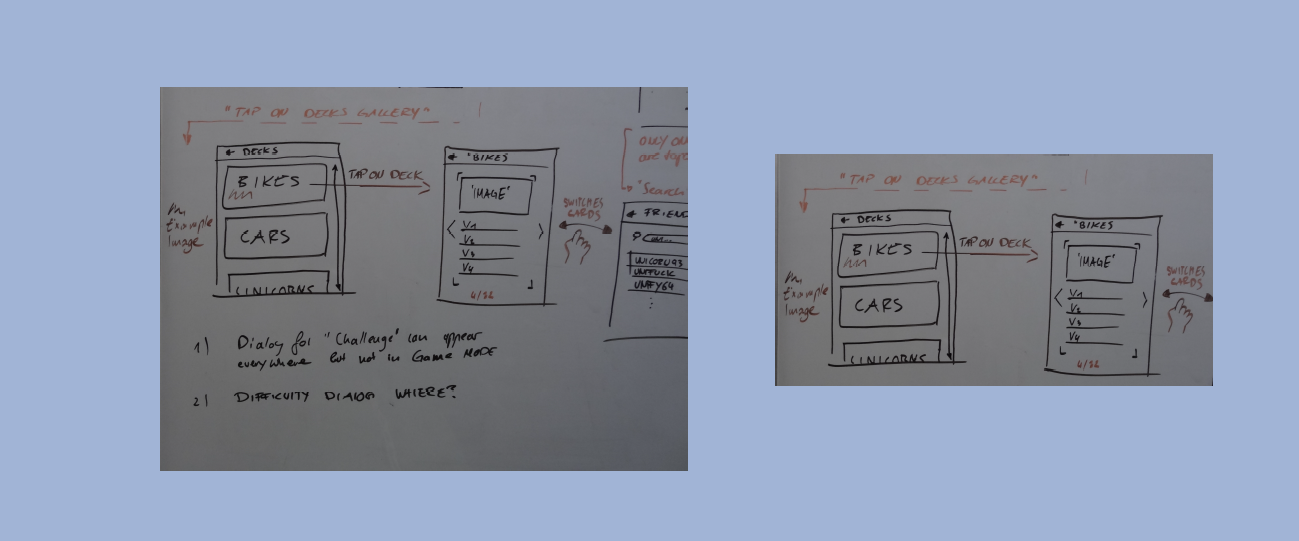
\includegraphics[scale=0.4]{pics/deckgallery.png}
	\caption{Kartenansicht/Kartengallerie}
	\label{DeckGallery}
\end{center}
In der Abbildung ~\ref{DeckGallery} wählt der Nutzer eines seiner Decks aus und kann sich dessen Karten ansehen.
\end{figure}

\begin{figure}[!ht]
\begin{center}
	\centering
	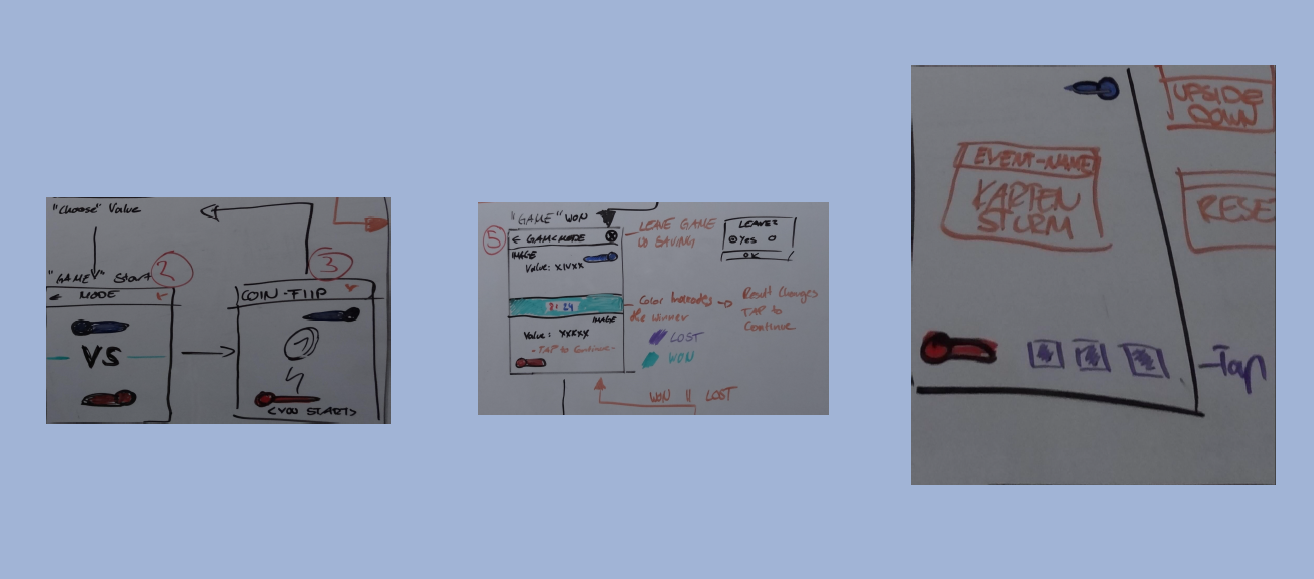
\includegraphics[scale=0.4]{pics/gameplay.png}
	\caption{Spielablauf}
	\label{gamePlay}
\end{center}
Diese Screens zeigen den grundlegenden Ablauf eines Spiel. Diese sind zwar unterschiedlich je nach Modi aber zum Zeitpunkt der Mockups ging es nur um ein generelles Darstellen des Prozesses.
~\ref{gamePlay} zeigt.
\end{figure}
\clearpage

\section{Implementierung}
\subsection{Ausgewählte Implementierungsdetails}
\subsubsection{Startseite | Profil}

\begin{figure}[!ht]
  \centering
  \begin{minipage}{0.45\textwidth}
    \centering
    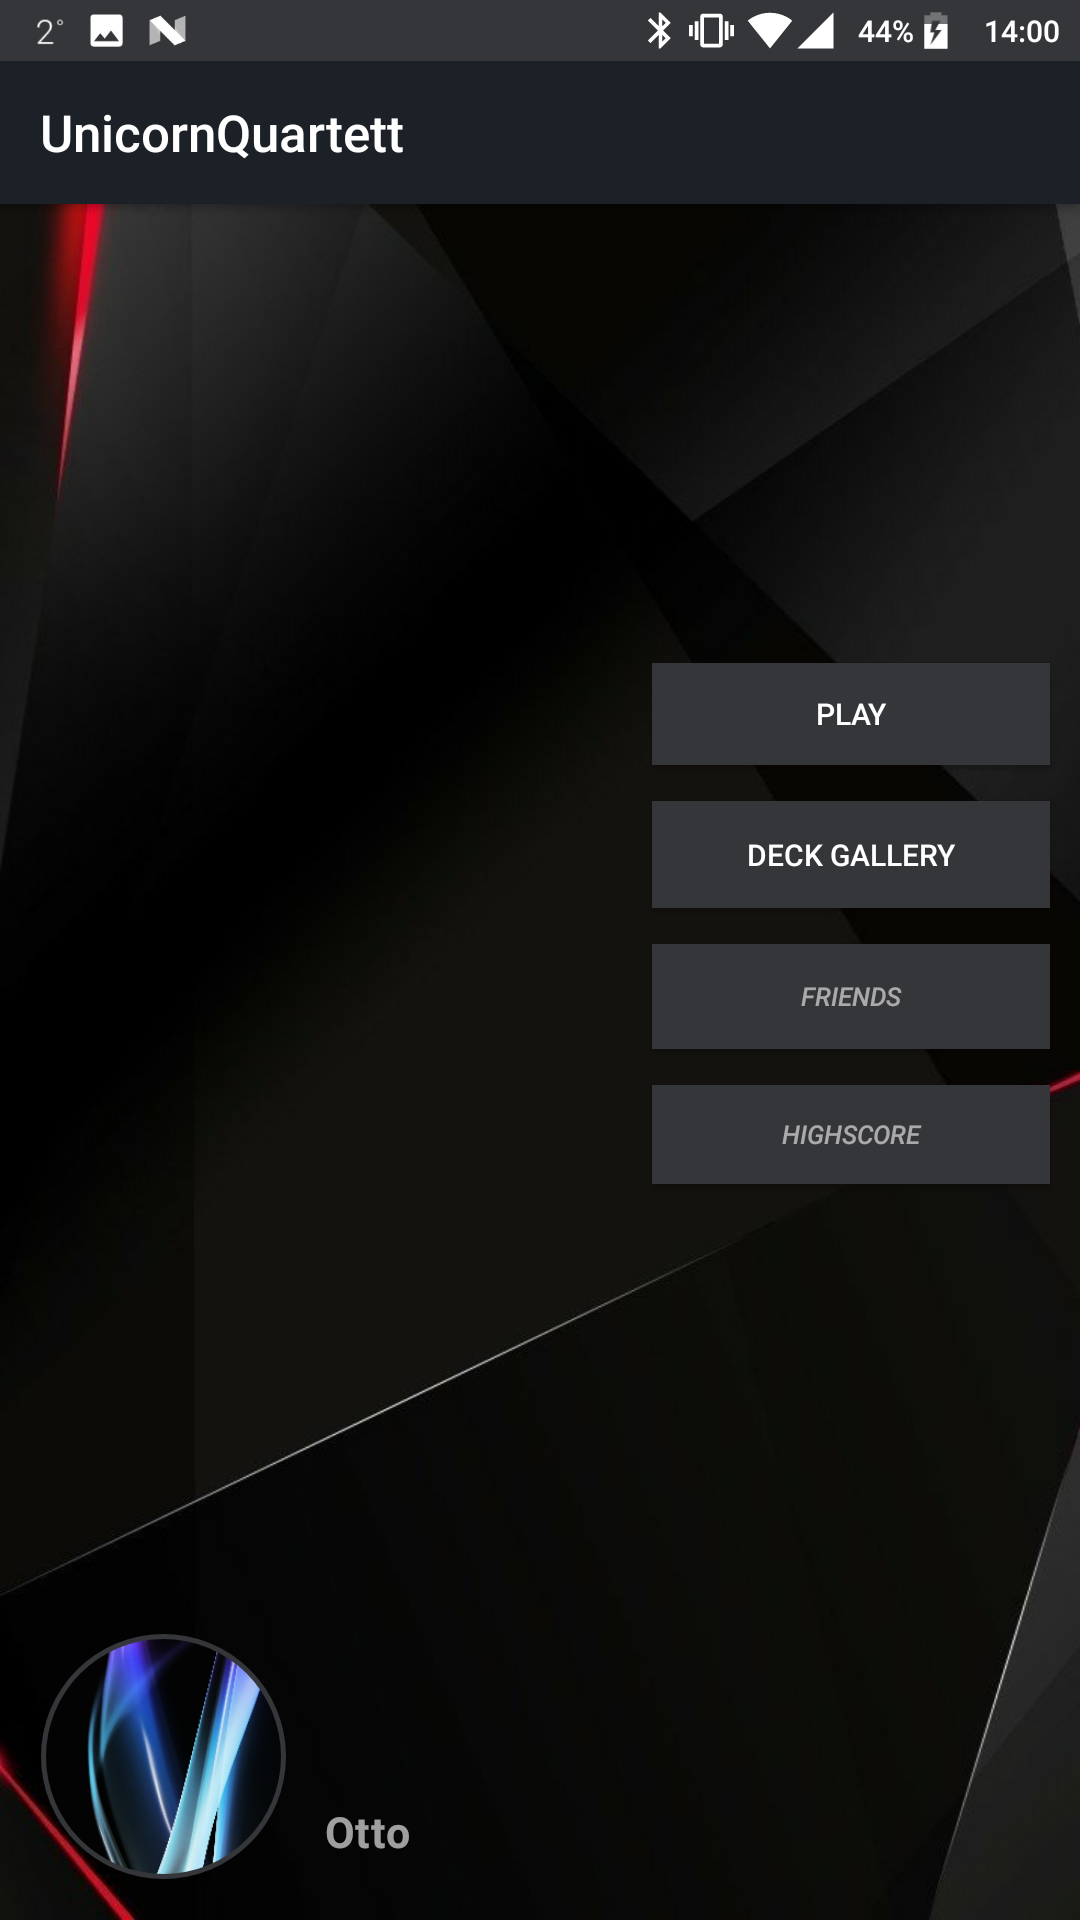
\includegraphics[width=4cm]{img/start.png}
    \caption{Startseite}
  \end{minipage}
  \hfill
  \begin{minipage}{0.45\textwidth}
    \centering
    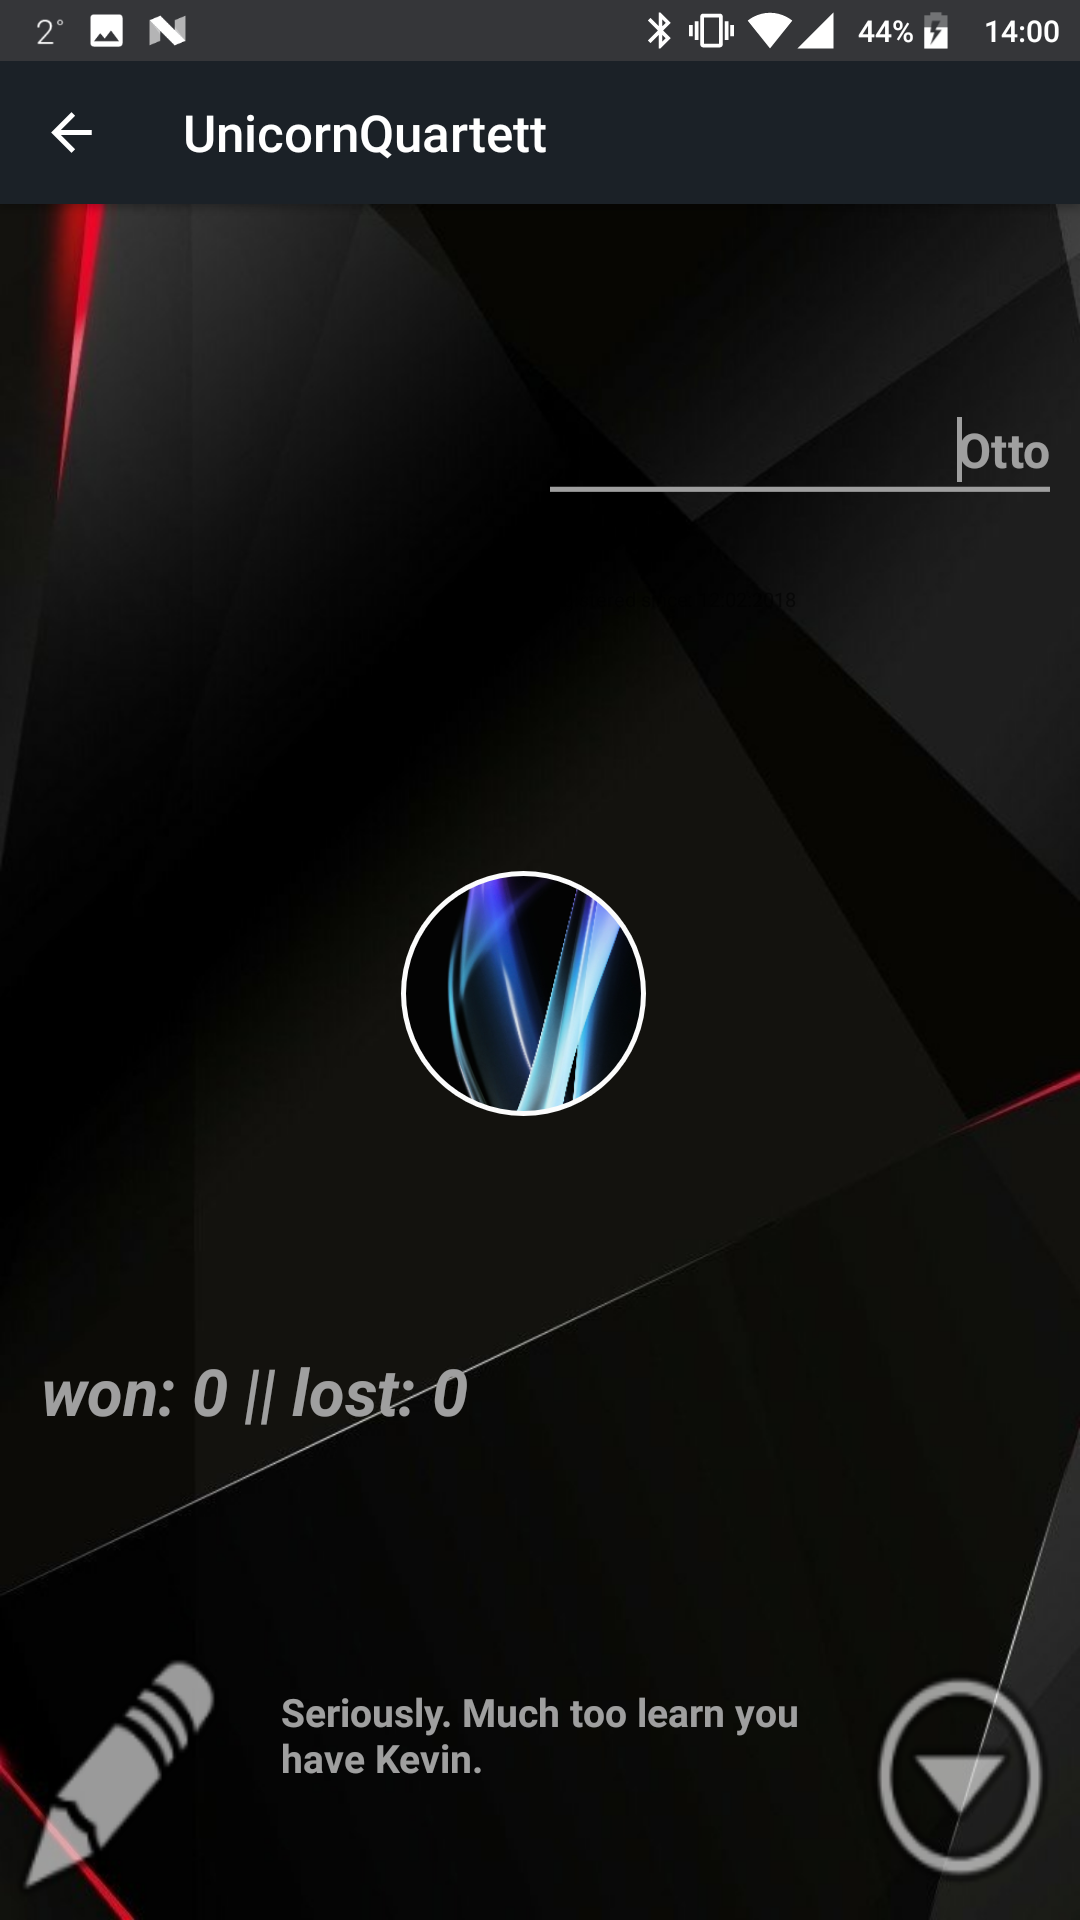
\includegraphics[width=4cm]{img/profile.png}
    \caption{Profil}
  \end{minipage}
\end{figure}

\noindent
Wenn der Nutzer das erste Mal die Anwendung startet, wird er aufgefordert, einen Benutzernamen einzugeben und ein Profilbild anzugeben. Zudem muss er sich für ein Darstellungsthema entscheiden.
Dieses kann er entweder mit der Kamera des Smartphones aufnehmen oder ein bereits erstelltes Bild aus der Galerie verwenden.
Das Profilbild wird nun in allen Übersichtsscreens am unterem linken Bildschirmrand angezeigt.
Beim erstmaligem Starten der Anwendung wird somit ein User Objekt angelegt, welches anschließend in der Realm Datenbank persitiert wird. \newline
Klickt der Nutzer auf sein Profilbild, kommt er zur Profilansicht. Dort kann er seinen Nutzernamen, das Profilbild und das Darstellungsthema ändern.
Zudem kann der Nutzer hier allerdings auch die Schwierigkeitsstufe der künstlichen Intelligenz auswählen. Er erhält weiterhin eine individuelle Übersicht einer internen Auswertung über seine gesamte Spielhistorie, 
welche abhängig von dem Verhältnis "Sieg - Niederlage" unterschiedliche Rückmeldungen an den Nutzer bietet.
All diese Konfigurationen werden in der Datenbank im User Eintrag hinterlegt und ggf. aktualisiert. Die Spielhistorie wird anhang von einer in der Datenbank hinterlegten Liste an Games analysiert.


\subsubsection{Deckansicht}
\begin{figure}[!ht]
\begin{center} 
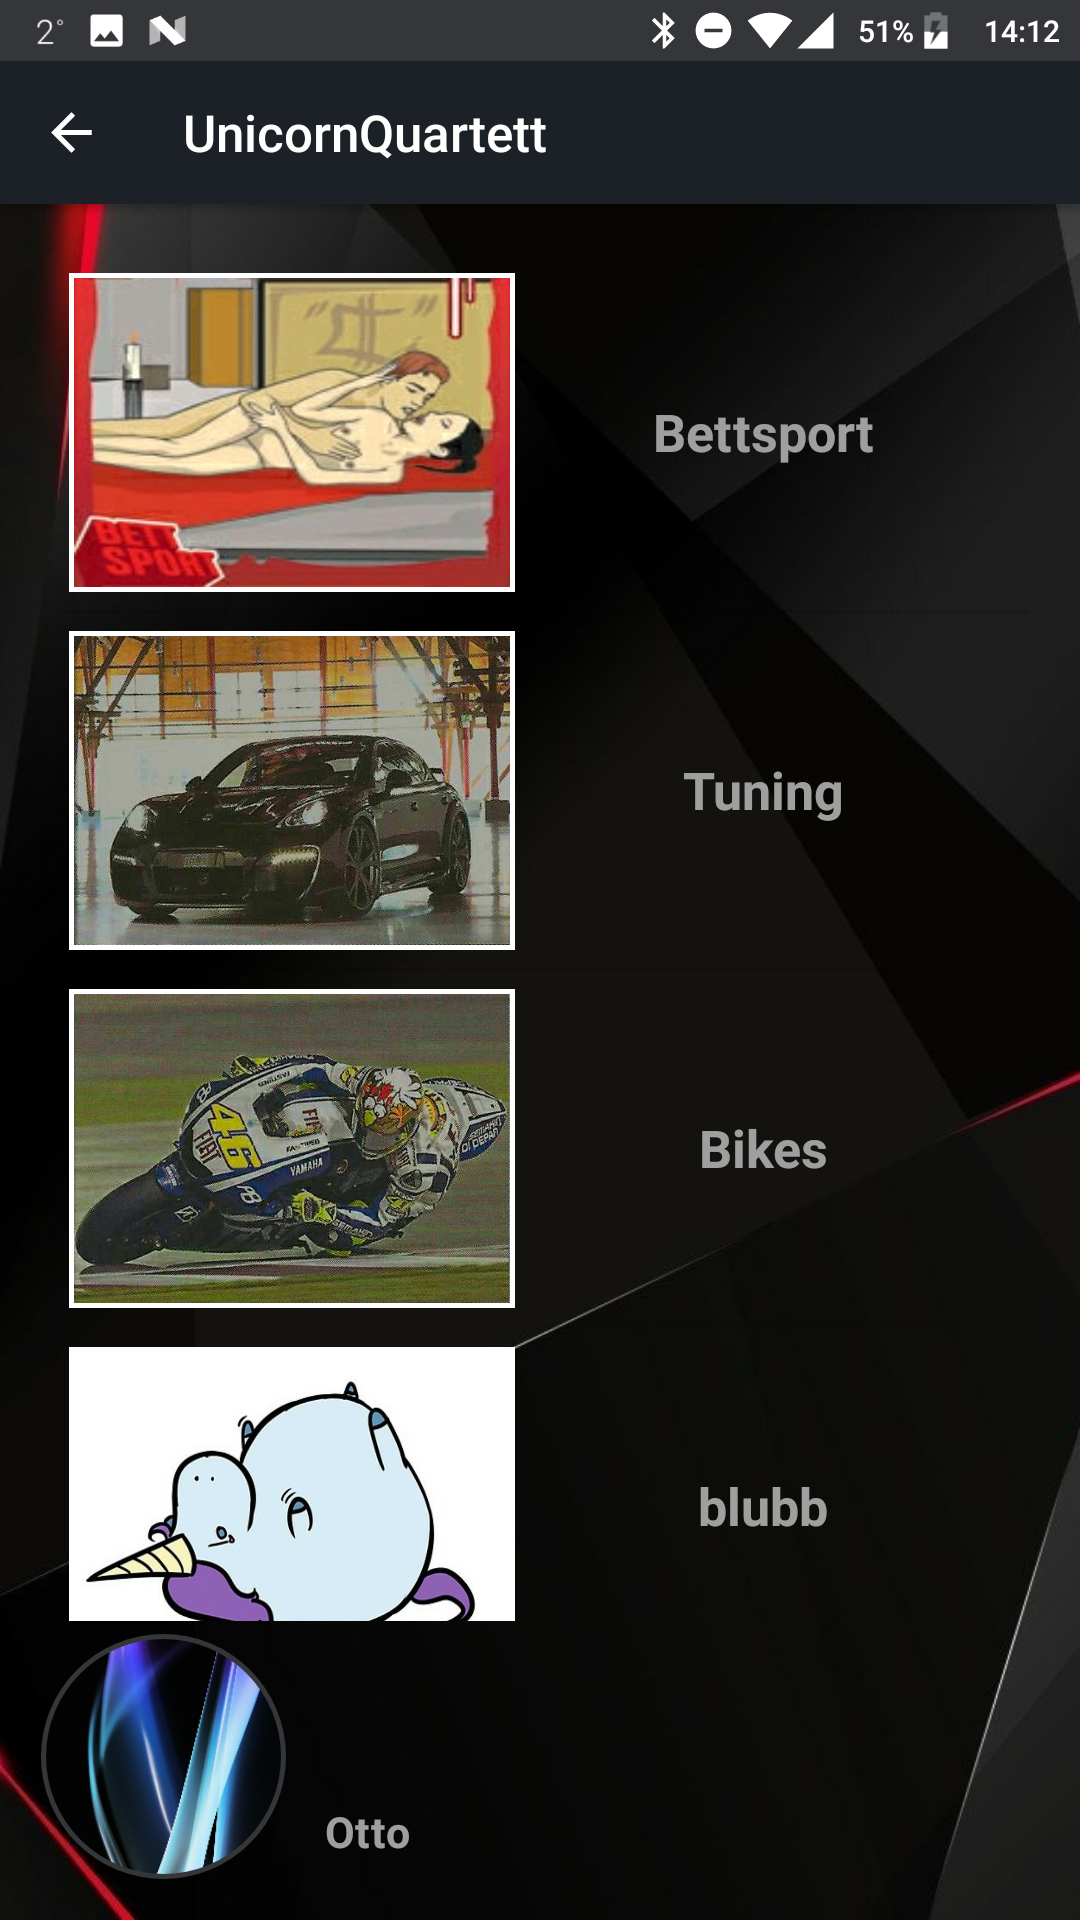
\includegraphics[scale=0.1]{img/deck.png}
    \caption{Gallerie}
\end{center}
\end{figure}

\ \newline
In der Deckansicht kann man alle zum Download stehenden bzw. bereits heruntergeladenen Decks einsehen. Beim Start der Activity wird überprüft, welche Decks auf dem Server zum Download verfügbar sind und welche davon bereits auf dem Endgerät heruntergeladen wurden.
Steht ein Deck zum Download bereit, kann auf den entsprechenden Platzhalter geklickt werden und der Download beginnt. Sämtliche Netzwerkaktionen wurden über Volley realisiert. Zudem kann ein Deck nur bei bestehender WLAN-Verbindung heruntergeladen werden. Sollte dies nicht der Fall sein, wird der Nutzer darüber informiert. Dabei werden nacheinander alle nötigen Informationen über das Deck, sein Attributschema und die
einzelnen Karten heruntergeladen und in temporäre Objekte zum Bauen von den tatsächlich in der Datenbank hinterlegten für das Spiel notwendingen Objekten zusammengefasst. Nach dem tatsächlichen Download werden aus diesen temporären BuildObjekten in einem weiteren Prozess die 
tatsächlichen Objekte für die Datenbank erstellt. Ist der Vorgang erfolgreich abgeschlossen, werden die temporären Dateien gelöscht und die Deckansicht refresht.
Während dem Entwicklungsprozess traten auf manchen Endgeräten immer wieder \textit{OutOfMemoryError}s auf. Um diese zu verhindern, musste jedes Bild über einen Algorithmus relativ zu seiner ursprünglichen Auflösung heruntergerendert werden.
Durch einen Klick auf ein heruntergeladenes Deck gelangt man in die Kartenansicht des Decks, in dem Karten des Decks inkl. ihrer Werte angezeigt werden.

\subsubsection{Das Spiel}
\begin{figure}[!ht]
  \centering
  \begin{minipage}{0.45\textwidth}
    \centering
    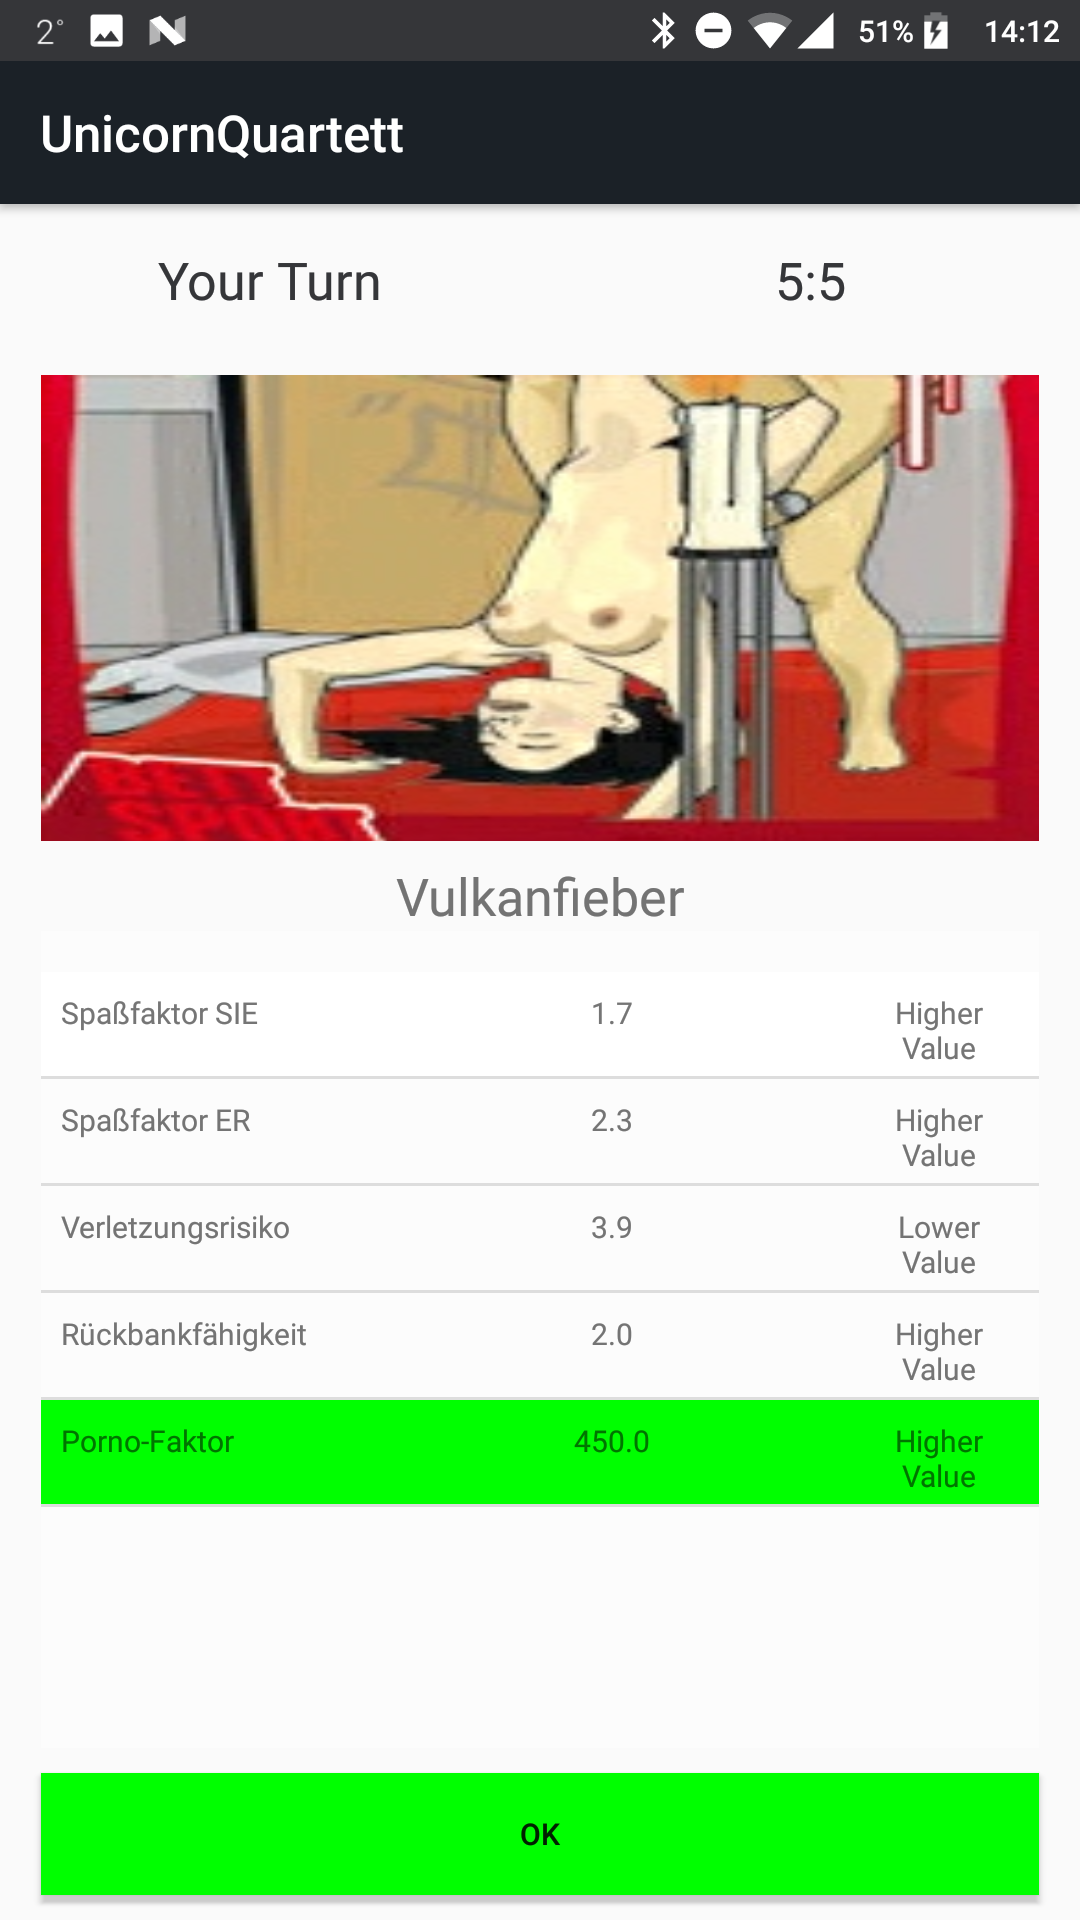
\includegraphics[width=4cm]{img/game.png}
    \caption{Das Spiel}
  \end{minipage}
  \hfill
  \begin{minipage}{0.45\textwidth}
    \centering
    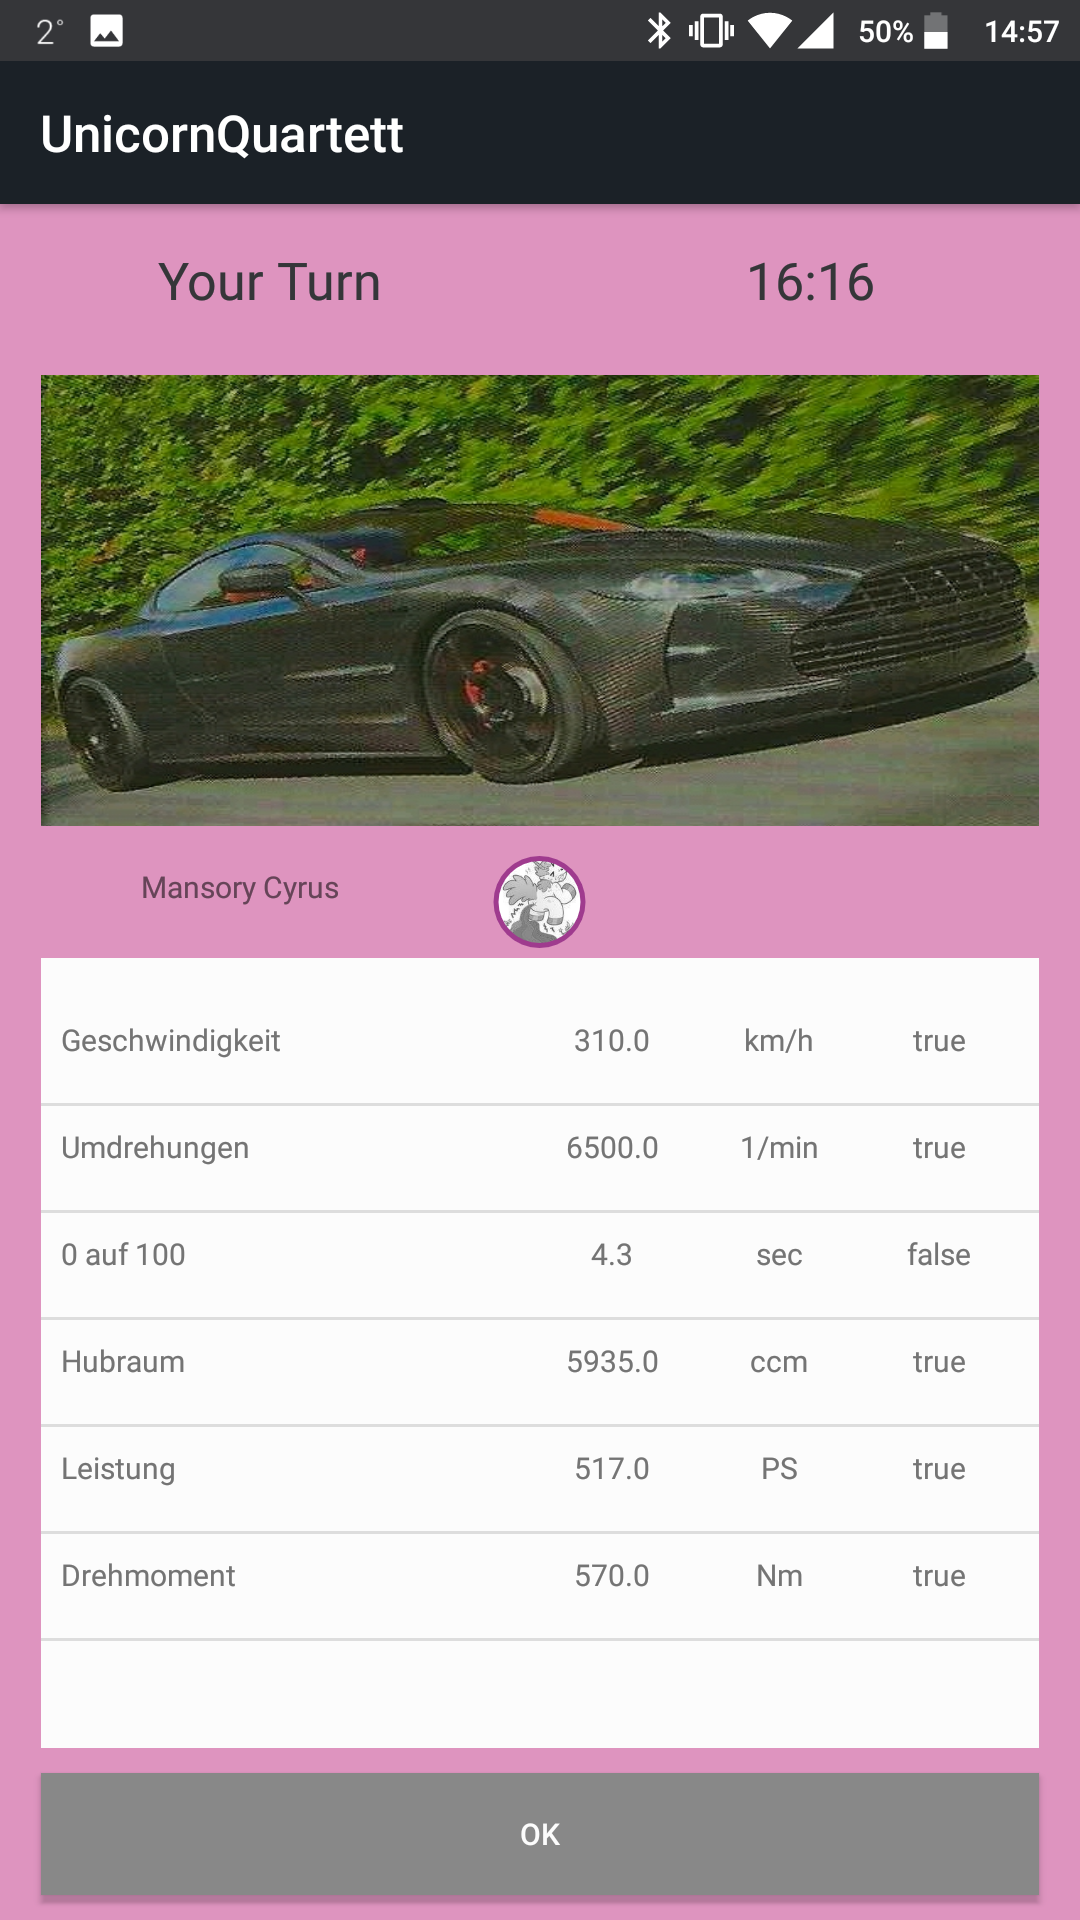
\includegraphics[width=4cm]{img/unicorn.png}
    \caption{Unicorn Modus}
  \end{minipage}
\end{figure}

\noindent
Der Nutzer kann zwischen zwei verschiedenen Spielmodi auswählen: Dem "normalen" Standard Modus und den speziellen Unicorn Modus.
Beide verfolgen grundlegend das gleiche Prinzip: Abwechselnd wählen die Kontrahenten einen Wert von ihrer Karte aus. Der Gewinner, also der Spieler mit dem besseren Wert, bekommt die Karte des Verlierers.
Dabei wird nach jeder Runde der aktuelle Zwischenstand, die jeweiligen Kartenstapel sowie der StichKartenStapel, der angelegt wird, sobald beide Spieler den gleichen Wert haben, in einem Game Objekt in der Datenbank hinterlegt.
Das heißt, dass jeder Zeit das aktuelle Spiel unterbrochen werden kann und erst später, auch nach dem Beenden der Anwendung, wieder an der gleichen Stelle fortgesetzt werden kann. Zudem hat der Nutzer die Möglichkeit, ein angefangenes Spiel zu löschen und
neu oder mit einem anderem Deck anzufangen.
\newline
Im Unicorn Modus hingegen beeinflussen zufällig generierte Events und vom Spieler eingesetzte Boni das Spielgeschehen. Das grundlegende Spielprinzip bleibt jedoch erhalten.
\newline
Die Implementierung der künstlichen Intelligenz hat sich sehr einfach gestaltet. Je nach Schwierigkeitsgrad entscheidet die KI zufällig oder aus einem Bereich der prozentual anhand dem Durchschnitt der Wertekategorien im Deck berechneten Werte.
Die KI kennt dabei wie ein menschlicher Spieler die Karten des Gegners nicht und kann somit nicht unfairer Weise strategische Entscheidungen bzgl. der Werte seines Gegners treffen.
 
\subsection{Architektur}
\subsubsection{Datenmodell}

\noindent
Das Datenmodell dieser Anwendung basiert auf REALM. Realm ist ein Datenbank Management System, welches insbesondere für mobile Plattformen wie Android gedacht ist. Realm bietet sich vor allem für objektorientiere Anwendungsansätze wie Android an, da
mithilfe von Realm sehr einfach Objekte abgebildet werden und diese ohne Mehraufwand seitens des Programmierers in die Datenbank gespeichert und wieder ausgelesen werden können. Realm bietet die Möglichkeit, Operationen auf einer Datenbank auszuführen, 
ohne klassische SQL Befehle einsetzen zu müssen. Diese werden implizit von Realm gehandhabt.

\subsubsection{Klassenstruktur}

\noindent
Bei der Implentierung wurde versucht, sich an das MVC Pattern zu halten. Dies gelang jedoch stellenweise nicht, weil aufgrund der fehlenden Erfahrung noch eine zu hohe Kopplung zwischen Views und Moduel in den Activities vorhanden ist.

\end{document}
